%  CONCLUSION au lieu de extension 

%% maybe add extension as a part of the conclusion for this chapter 
\section{Conclusion \note{Uncomplete }}
In this chapter we :
- studied two aspects of the three creterias of the emperical research and how they will be applied in the field of energy measurement .
- we provided a brief comparaison of different methods to increase the reproducibility of the measurement .
- we studied the factors that can affect the measurement accuracy and how to reduce them .
- and finally



%  THIS SHOULD BE WITHIN THE perspective chapter 
% By the end of this study, we have gathered enough guidelines to make the tests more reproducible, accurate and extensible.
% We created a set of new tests named \textbf{energy tests} which are more similar to performance tests.
% Thanks to the work of two interns [Mamadou and Adrien] we created a CI/CD platform to measure the energy consumption of Java projects and we could track the evolution of the this energy across different stages of the project.
% In the figure below we see an example of this plugin.
% For more details please visit the gitlab repository\footnote{\url{https://gitlab.inria.fr/mamdiall/J-Joules}}~\footnote{\url{https://gitlab.inria.fr/mamdiall/jjoules-plugin}} .





% \begin{figure}%[!htb]
%     \center{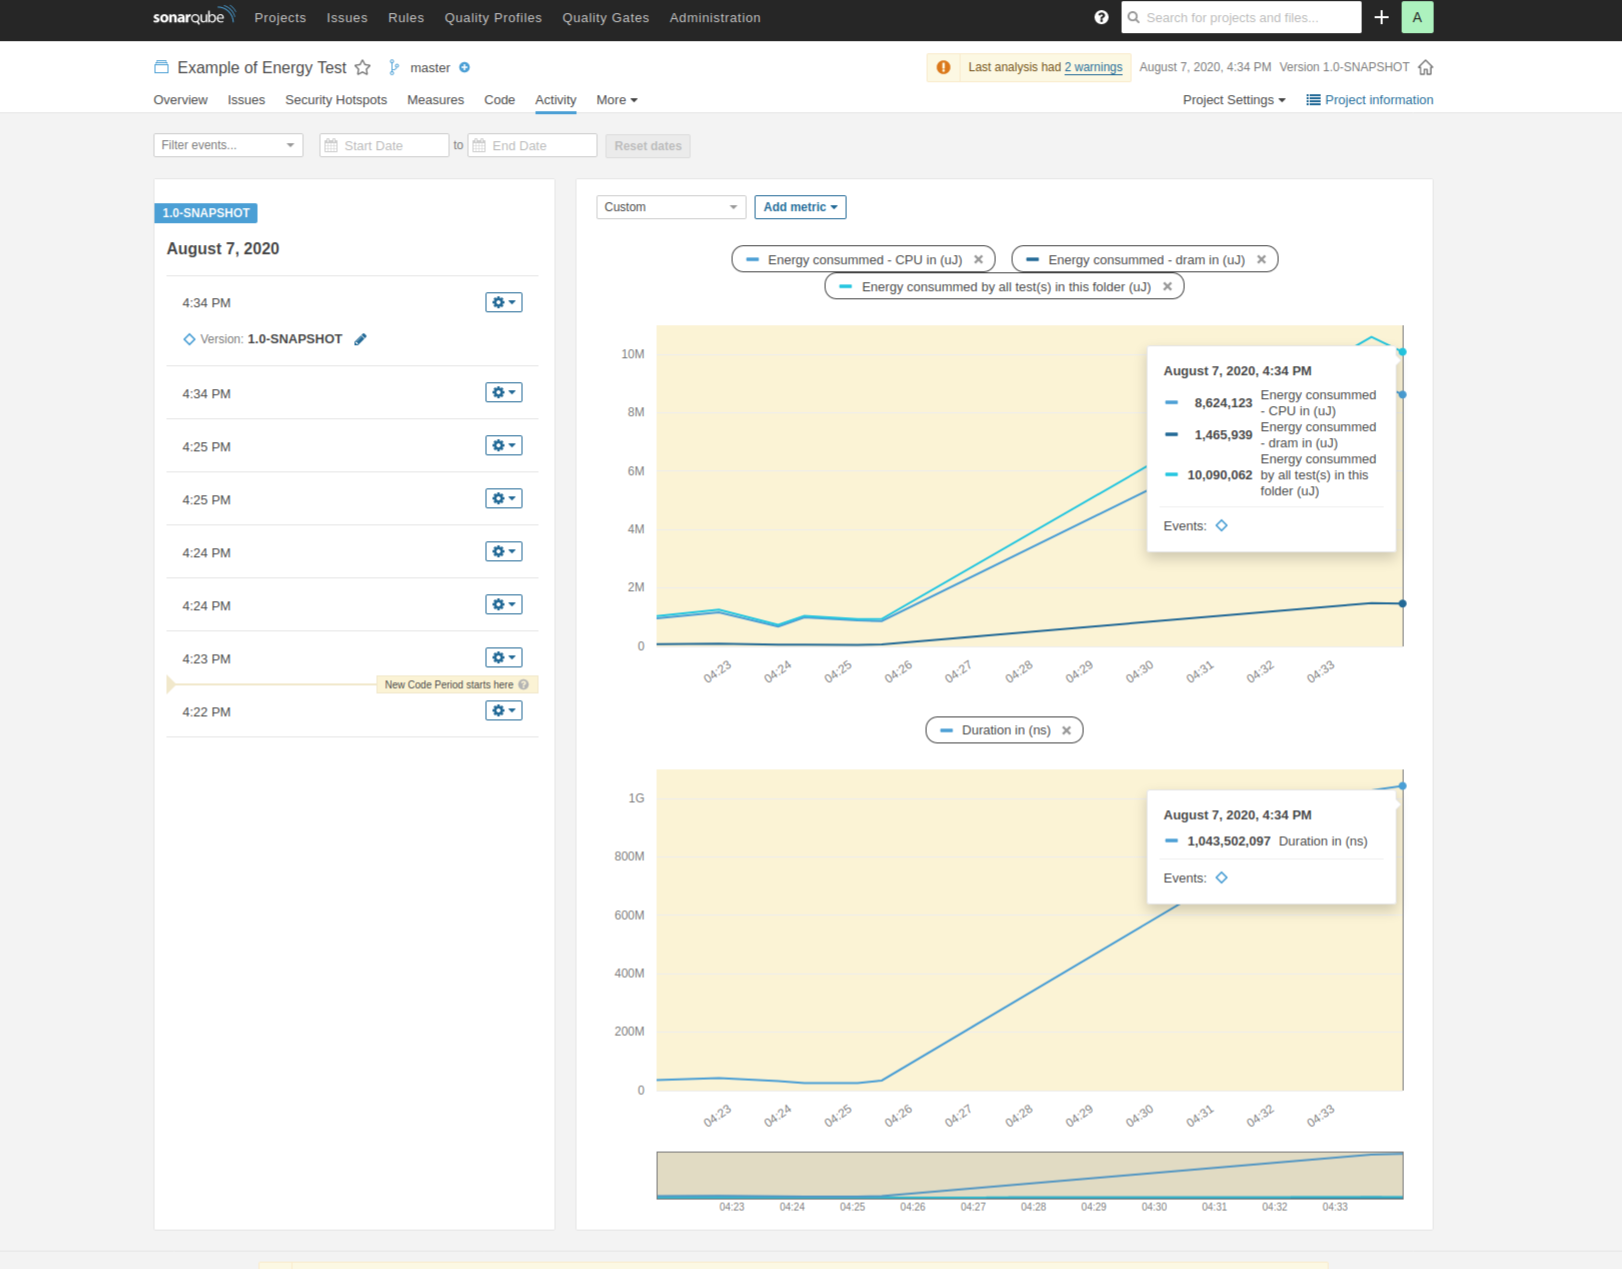
\includegraphics[width=.9\linewidth]{imgs/JunitSonarplugin}}
%     \caption{Example of the Junit Sonar Plugin}\label{fig:sonar_plugin}
% \end{figure}
